% EGE 2027, task 9. Source IDs and URLs are kept in comments.
% Editable task bank. Append new BankTask blocks at the end of the document.
\documentclass[12pt,a4paper]{article}
\usepackage{physics-textbook}
\usepackage{graphicx,needspace}
\newif\ifShowSolutions
\ifdefined\TutorEdition
  \ShowSolutionstrue
\else
  \ShowSolutionsfalse
\fi
\newcounter{banktask}
\newcommand{\BankTask}[3]{%
  \refstepcounter{banktask}%
  \Needspace{35mm}\par\medskip\noindent\begin{minipage}{\linewidth}%
  \noindent\textbf{\thebanktask.}\quad #2\par
  \ifShowSolutions
    #3\par
    \ifdefined\TutorEdition
      \ifcsname TutorSource#1\endcsname
        \smallskip{\small\csname TutorSource#1\endcsname\par}%
      \fi
    \fi
  \fi
  \end{minipage}\par\medskip
}
\begin{document}
Справочные величины (если в условии не оговорено иное):\par
$M_{\mathrm{He}}=4\,\text{г}/\text{моль}$\par
$M_{\mathrm{Ar}}=40\,\text{г}/\text{моль}$



% Source c17D9F: https://ege.fipi.ru/bank/questions.php?search=1&proj=BA1F39653304A5B041B656915DC36B38&qid=c17D9F
\BankTask{c17D9F}{
В вертикальном цилиндре под поршнем находится \(1\,\text{моль}\) гелия. Поршень может перемещаться в сосуде без трения. Атмосферное давление считать постоянным. Масса гелия в сосуде не изменяется.
\begin{enumerate}
\item При медленном понижении температуры объём, занимаемый гелием, не изменяется.
\item При медленном понижении температуры давление гелия не изменяется.
\item Если на поршень насыпать некоторое количество песка, не меняя температуры гелия, то после установления равновесия в системе давление гелия будет меньше первоначального давления.
\item При медленном повышении температуры сила давления гелия на поршень не изменяется.
\item При медленном изотермическом сжатии гелия в цилиндре он отдаёт окружающим телам некоторое положительное количество теплоты.
\end{enumerate}
}{
\smallskip\noindent\textbf{Решение от GPT}\par
В равновесии \(p=p_{\text{атм}}+Mg/S\), где \(M\) — масса поршня с нагрузкой, \(S\) — площадь поршня.
\begin{enumerate}
\item Неверно: при постоянной нагрузке \(p=\mathrm{const}\), поэтому из \(pV=\nu RT\) следует, что при охлаждении объём уменьшается.
\item Верно: давление определяется неизменной нагрузкой и атмосферным давлением.
\item Неверно: добавление песка увеличивает \(M\), поэтому давление возрастает.
\item Верно: сила давления \(F=pS\) постоянна.
\item Верно: при изотермическом сжатии \(\Delta U=0\), работа газа \(A<0\); следовательно, \(Q=\Delta U+A<0\), газ отдаёт теплоту.
\end{enumerate}
Ответ: \(245\).
}

% Source 430072: https://ege.fipi.ru/bank/questions.php?search=1&proj=BA1F39653304A5B041B656915DC36B38&qid=430072
\BankTask{430072}{
Относительная влажность воздуха в закрытом сосуде с поршнем равна \(40\,\%\). Объём сосуда за счёт движения поршня медленно уменьшают при постоянной температуре. В конечном состоянии объём сосуда в \(4\) раза меньше начального.
\begin{enumerate}
\item При уменьшении объёма сосуда в \(2{,}5\) раза на стенках появляется роса.
\item Давление пара в сосуде всё время увеличивается.
\item В конечном и начальном состояниях масса пара в сосуде одинакова.
\item При уменьшении объёма в \(2\) раза относительная влажность воздуха в сосуде стала равна \(80\,\%\).
\item В конечном состоянии весь пар в сосуде сконденсировался.
\end{enumerate}
}{
\smallskip\noindent\textbf{Решение от GPT}\par
При постоянной температуре давление насыщенного пара \(p_{\text{нас}}\) постоянно. До насыщения \(pV=\mathrm{const}\), поэтому \(\varphi=0{,}4V_0/V\).
\begin{enumerate}
\item Верно: насыщение достигается при \(V=0{,}4V_0=V_0/2{,}5\); начинается выпадение росы.
\item Неверно: после насыщения давление пара остаётся равным \(p_{\text{нас}}\).
\item Неверно: часть пара конденсируется. При \(V_f=V_0/4\) отношение масс пара равно \(m_f/m_0=(1/4)/0{,}4=0{,}625\).
\item Верно: при \(V=V_0/2\) влажность \(\varphi=0{,}8=80\,\%\).
\item Неверно: в конечном состоянии остаётся насыщенный пар.
\end{enumerate}
Ответ: \(14\).
}

% Source 35852E: https://ege.fipi.ru/bank/questions.php?search=1&proj=BA1F39653304A5B041B656915DC36B38&qid=35852E
\BankTask{35852E}{
Горячее вещество, первоначально находившееся в жидком состоянии, медленно охлаждали. Мощность теплоотвода постоянна. В таблице приведены результаты измерений температуры вещества с течением времени.
\begin{center}
\begin{tabular}{|l|r|r|r|r|r|r|r|r|}
\hline
Время, $\text{мин}$ & \(0\) & \(5\) & \(10\) & \(15\) & \(20\) & \(25\) & \(30\) & \(35\) \\
\hline
Температура, \({}^{\circ}\mathrm{C}\) & \(250\) & \(242\) & \(234\) & \(232\) & \(232\) & \(232\) & \(230\) & \(216\) \\
\hline
\end{tabular}
\end{center}
\begin{enumerate}
\item Температура плавления вещества в данных условиях равна \(232\,{}^{\circ}\mathrm{C}\).
\item Через \(20\,\text{мин}\). после начала измерений вещество находилось только в твёрдом состоянии.
\item Удельная теплоёмкость вещества в жидком и твёрдом состояниях одинакова.
\item Через \(30\,\text{мин}\). после начала измерений вещество находилось только в твёрдом состоянии.
\item Процесс кристаллизации вещества занял более \(25\,\text{мин}\).
\end{enumerate}
}{
\smallskip\noindent\textbf{Решение от GPT}\par
\begin{enumerate}
\item Верно: участок постоянной температуры соответствует кристаллизации, поэтому \(T_{\text{пл}}=232\,{}^{\circ}\mathrm{C}\).
\item Неверно: в момент \(t=20\,\text{мин}\) идёт кристаллизация, присутствуют жидкая и твёрдая фазы.
\item Неверно: при постоянной мощности \(P=mc\lvert\Delta T/\Delta t\rvert\). Скорости охлаждения жидкости и твёрдого вещества равны соответственно \(8/5=1{,}6\) и \(14/5=2{,}8\,{}^{\circ}\mathrm{C}/\text{мин}\); теплоёмкости различны.
\item Верно: через \(30\,\text{мин}\) температура \(230\,{}^{\circ}\mathrm{C}\) ниже температуры кристаллизации, вещество полностью затвердело.
\item Неверно: кристаллизация началась после \(10\,\text{мин}\) и завершилась до \(30\,\text{мин}\), поэтому её длительность меньше \(20\,\text{мин}\).
\end{enumerate}
Ответ: \(14\).
}

% Source E27EA7: https://ege.fipi.ru/bank/questions.php?search=1&proj=BA1F39653304A5B041B656915DC36B38&qid=E27EA7
\BankTask{E27EA7}{
При изучении процессов, происходящих с гелием, ученик занёс в таблицу результаты измерения температуры и давления одного и того же количества газа в различных равновесных состояниях. Газ считать идеальным.
\begin{center}
\begin{tabular}{|c|c|c|c|c|c|c|c|}
\hline
№ состояния & 1 & 2 & 3 & 4 & 5 & 6 & 7 \\
\hline
$p,\,\text{кПа}$ & $100$ & $90$ & $75$ & $50$ & $55$ & $75$ & $100$ \\
\hline
$t$, ${}^{\circ}\mathrm{C}$ & $27$ & $27$ & $27$ & $27$ & $57$ & $177$ & $327$ \\
\hline
\end{tabular}
\end{center}
\begin{enumerate}
\item Объём газа в состоянии $4$ в $2$ раза меньше объёма газа в состоянии $1$.
\item В состояниях $4$--$7$ объём газа был одинаковым.
\item Внутренняя энергия газа в состоянии $6$ в $3$ раза больше, чем в состоянии $5$.
\item При переходе от состояния $2$ к состоянию $3$ в ходе изотермического процесса газ получал тепло.
\item При переходе от состояния $5$ к состоянию $6$ в ходе изохорного процесса газ совершал работу.
\end{enumerate}
}{
\smallskip\noindent\textbf{Решение от GPT}\par
Для данного количества газа $V=\nu RT/p$, а для гелия $U=\frac32\nu RT$. Температуры состояний: $300$, $300$, $300$, $300$, $330$, $450$, $600\ \text{К}$.
\begin{enumerate}
\item Неверно: $V_4/V_1=p_1/p_4=2$, то есть объём больше в $2$ раза.
\item Верно: $T_4/p_4=T_5/p_5=T_6/p_6=T_7/p_7=6\ \text{К}/\text{кПа}$, поэтому объёмы одинаковы.
\item Неверно: $U_6/U_5=T_6/T_5=450/330=15/11\ne3$.
\item Верно: при постоянной температуре давление уменьшается, газ расширяется; $\Delta U=0$, $Q=A>0$.
\item Неверно: при изохорном процессе $A=0$.
\end{enumerate}
Ответ: $24$.
}

% Source 84BDA5: https://ege.fipi.ru/bank/questions.php?search=1&proj=BA1F39653304A5B041B656915DC36B38&qid=84BDA5
\BankTask{84BDA5}{
Сосуд разделён на две равные по объёму части пористой неподвижной перегородкой. В левой части сосуда содержится $8\ \text{г}$ гелия, в правой --- $1\ \text{моль}$ аргона. Перегородка может пропускать молекулы гелия и является непроницаемой для молекул аргона. Температура газов одинакова и остаётся постоянной.
Рассматривается состояние газов после установления равновесия в системе.
\begin{enumerate}
\item Давление в обеих частях сосуда одинаково.
\item Концентрация гелия и аргона в правой части сосуда одинакова.
\item Внутренняя энергия гелия в сосуде больше, чем внутренняя энергия аргона.
\item Внутренняя энергия гелия в сосуде в конечном состоянии больше, чем в начальном.
\item В правой части сосуда общее число молекул газов в $2$ раза меньше, чем в левой части.
\end{enumerate}
}{
\smallskip\noindent\textbf{Решение от GPT}\par
Молярная масса гелия $M_{\mathrm{He}}=4\ \text{г/моль}$, поэтому $\nu_{\mathrm{He}}=8/4=2\ \text{моль}$. В равновесии концентрация гелия одинакова в обеих частях: в каждой находится по $1\ \text{моль}$ гелия. Весь аргон ($1\ \text{моль}$) остаётся справа. Пусть объём каждой части равен $V$.
\begin{enumerate}
\item Неверно: $p_{\text{лев}}=\dfrac{(1\ \text{моль})RT}{V}$, $p_{\text{прав}}=2p_{\text{лев}}$.
\item Верно: справа количества гелия и аргона равны, поэтому равны и их концентрации.
\item Верно: оба газа одноатомные, $U=\frac32\nu RT$; следовательно, $U_{\mathrm{He}}/U_{\mathrm{Ar}}=2$.
\item Неверно: количество гелия и его температура не изменились, поэтому его внутренняя энергия постоянна.
\item Неверно: справа общее число молекул в $2$ раза больше, чем слева.
\end{enumerate}
Ответ: $23$.
}

% Source DE8B36: https://ege.fipi.ru/bank/questions.php?search=1&proj=BA1F39653304A5B041B656915DC36B38&qid=DE8B36
\BankTask{DE8B36}{
В понедельник и вторник температура воздуха была одинаковой. Парциальное давление водяного пара в атмосфере в понедельник было меньше, чем во вторник.
\begin{enumerate}
\item Масса водяных паров, содержащихся с $1\ \text{м}^{3}$ воздуха в понедельник была больше, чем во вторник
\item Относительная влажность воздуха в понедельник была меньше, чем во вторник
\item Концентрация молекул водяного пара в воздухе в понедельник и вторник была одинаковой
\item Давление насыщенных водяных паров в понедельник было больше, чем во вторник
\item Плотность водяных паров, содержащихся в воздухе в понедельник была меньше, чем во вторник
\end{enumerate}
}{
\smallskip\noindent\textbf{Решение от GPT}\par
При одинаковой температуре $p_{\text{нас}}(T)$ одинаково в оба дня. По формулам $\varphi=p/p_{\text{нас}}$, $n=p/(kT)$ и $\rho=Mp/(RT)$ меньшему парциальному давлению соответствуют меньшие влажность, концентрация и плотность пара.
\begin{enumerate}
\item Неверно: масса пара в $1\ \text{м}^{3}$ в понедельник меньше.
\item Верно: $\varphi_{\text{пн}}<\varphi_{\text{вт}}$.
\item Неверно: $n_{\text{пн}}<n_{\text{вт}}$.
\item Неверно: давления насыщенного пара одинаковы.
\item Верно: $\rho_{\text{пн}}<\rho_{\text{вт}}$.
\end{enumerate}
Ответ: $25$.
}

% Source 403D76: https://ege.fipi.ru/bank/questions.php?search=1&proj=BA1F39653304A5B041B656915DC36B38&qid=403D76
\BankTask{403D76}{
В двух сосудах одинакового объёма находятся разреженные газы.
В первом сосуде находится \(2\,\text{моль}\) гелия при температуре \(127\,^{\circ}\mathrm{C}\), во втором сосуде находится \(1\,\text{моль}\) аргона при температуре \(300\,\text{К}\).
\begin{enumerate}
\item Абсолютная температура газа во втором сосуде выше, чем в первом.
\item Среднеквадратичная скорость молекул газа в первом сосуде больше, чем во втором.
\item Давления газов в сосудах одинаковы.
\item Концентрация газа в первом сосуде в \(2\) раза меньше, чем во втором.
\item Отношение средней кинетической энергии теплового движения молекул аргона к средней кинетической энергии теплового движения молекул гелия равно \(0{,}75\).
\end{enumerate}
}{
\smallskip\noindent\textbf{Решение от GPT}\par
\(T_1=127+273=400\,\text{К}\), \(T_2=300\,\text{К}\).
\begin{enumerate}
\item Неверно: \(T_2<T_1\).
\item Верно: \(v_{\text{кв}}=\sqrt{3RT/M}\); у гелия температура выше, а молярная масса меньше, поэтому \(v_{\text{кв},1}>v_{\text{кв},2}\).
\item Неверно: \(p_1/p_2=\nu_1T_1/(\nu_2T_2)=8/3\).
\item Неверно: при одинаковых объёмах \(n_1/n_2=\nu_1/\nu_2=2\), то есть концентрация в первом сосуде больше.
\item Верно: \(\overline E=3kT/2\), поэтому \(\overline E_{\mathrm{Ar}}/\overline E_{\mathrm{He}}=300/400=0{,}75\).
\end{enumerate}
Ответ: \(25\).
}

% Source 0443DE: https://ege.fipi.ru/bank/questions.php?search=1&proj=BA1F39653304A5B041B656915DC36B38&qid=0443DE
\BankTask{0443DE}{
Герметичный теплоизолированный сосуд разделили неподвижной перегородкой, способной проводить тепло, на две равные части. В первую часть сосуда поместили некоторое количества аргона при температуре \(328\,\text{К}\), а во вторую --- такое же количество аргона при температуре \(15\,^{\circ}\mathrm{C}\).
Теплоёмкость сосуда пренебрежимо мала.
Рассматриваются изменения, происходящие с аргоном при переходе к тепловому равновесию.
\begin{enumerate}
\item Температура газа во второй части сосуда повысилась.
\item Внутренняя энергия газа в первой части сосуда увеличилась.
\item При теплообмене газ в первой части сосуда отдавал теплоту, а газ во второй части сосуда её получал.
\item Через достаточно большой промежуток времени температура газов в обеих частях сосуда стала одинаковой и равной \(25\,^{\circ}\mathrm{C}\).
\item В результате теплообмена газ в первой части сосуда совершил положительную работу.
\end{enumerate}
}{
\smallskip\noindent\textbf{Решение от GPT}\par
Начальная температура во второй части \(T_2=15+273=288\,\text{К}\). Объёмы постоянны, поэтому работа каждого газа \(A=0\). По закону сохранения энергии для равных количеств одного газа
\[
T_{\text{равн}}=\frac{328+288}{2}=308\,\text{К}=35\,^{\circ}\mathrm{C}.
\]
\begin{enumerate}
\item Верно: температура второго газа повысилась от \(288\) до \(308\,\text{К}\).
\item Неверно: \(U=\frac32\nu RT\), поэтому при охлаждении первого газа его внутренняя энергия уменьшилась.
\item Верно: теплота передавалась от более горячего первого газа ко второму.
\item Неверно: равновесная температура равна \(35\,^{\circ}\mathrm{C}\).
\item Неверно: при неподвижной перегородке \(A=0\).
\end{enumerate}
Ответ: \(13\).
}

% Source 12DC5B: https://ege.fipi.ru/bank/questions.php?search=1&proj=BA1F39653304A5B041B656915DC36B38&qid=12DC5B
\BankTask{12DC5B}{
В сосуде под поршнем при комнатной температуре долгое время находится вода и водяной пар. Масса воды равна массе пара. Объём сосуда медленно изотермически увеличивают в \(3\) раза.
\begin{enumerate}
\item Масса пара в сосуде не изменяется.
\item В конечном состоянии давление пара в сосуде в \(3\) раза меньше первоначального.
\item Давление пара сначала было постоянным, а затем стало уменьшаться.
\item Плотность пара в начале и конце опыта одинакова.
\item Концентрация пара в сосуде в начале опыта больше, чем в конце опыта.
\end{enumerate}
}{
\smallskip\noindent\textbf{Решение от GPT}\par
Первоначально пар насыщенный. Пока вода испаряется, при постоянной температуре давление и плотность пара постоянны. Обозначим начальную массу пара через \(m\), начальный объём сосуда через \(V\). Пренебрегая объёмом жидкости, полное испарение воды происходит при объёме \(2V\); далее пар становится ненасыщенным. В конце
\[
m_{\text{п},f}=2m,\qquad
\frac{\rho_f}{\rho_i}=\frac{2m/(3V)}{m/V}=\frac23,\qquad
\frac{p_f}{p_i}=\frac{n_f}{n_i}=\frac23.
\]
\begin{enumerate}
\item Неверно: масса пара увеличилась в \(2\) раза.
\item Неверно: давление уменьшилось примерно в \(1{,}5\) раза.
\item Верно: сначала пар оставался насыщенным, затем его давление уменьшалось.
\item Неверно: конечная плотность пара меньше начальной.
\item Верно: концентрация пропорциональна плотности, поэтому \(n_i>n_f\).
\end{enumerate}
Ответ: \(35\).
}

% Source 055098: https://ege.fipi.ru/bank/questions.php?search=1&proj=BA1F39653304A5B041B656915DC36B38&qid=055098
\BankTask{055098}{
Стальную кастрюлю, наполовину заполненную водой, поставили на плиту, закрыли лёгкой крышкой и стали нагревать воду до кипения. Атмосферное давление составляет \(760\,\text{мм рт. ст.}\)
\begin{enumerate}
\item Относительная влажность воздуха под крышкой в процессе нагревания воды уменьшается.
\item Внутренняя энергия водяного пара в кастрюле в процессе нагревания воды увеличивается.
\item При нагревании воды выше \(80\,^{\circ}\mathrm{C}\), когда схлопываются образующиеся пузырьки, давление водяных паров постепенно уменьшается.
\item Температура дна кастрюли вблизи границы с водой при кипении немного превышает \(100\,^{\circ}\mathrm{C}\).
\item Плотность насыщенных водяных паров над поверхностью воды в процессе её нагревания до температуры кипения увеличивается.
\end{enumerate}
}{
\smallskip\noindent\textbf{Решение от GPT}\par
1) Неверно: под крышкой воздух насыщается водяным паром, его относительная влажность не уменьшается.

2) Верно: при нагревании растут температура и количество водяного пара, поэтому его внутренняя энергия увеличивается.

3) Неверно: давление насыщенного пара с повышением температуры увеличивается; пузырьки схлопываются при попадании в более холодные слои воды вследствие конденсации пара.

4) Верно: при данном атмосферном давлении вода кипит при \(100\,^{\circ}\mathrm{C}\); для передачи теплоты от дна воде температура дна должна быть немного выше.

5) Верно: плотность насыщенного водяного пара увеличивается с температурой.

Ответ: \(245\).
}

% Source 2CEC9C: https://ege.fipi.ru/bank/questions.php?search=1&proj=BA1F39653304A5B041B656915DC36B38&qid=2CEC9C
\BankTask{2CEC9C}{
Объём сосуда, содержащего \(1\,\text{моль}\) неона, уменьшили вдвое и добавили в сосуд \(1\,\text{моль}\) гелия. Температура в сосуде поддерживается постоянной.
\begin{enumerate}
\item Концентрации неона и гелия в сосуде одинаковы.
\item Внутренняя энергия неона уменьшилась.
\item Плотность газа в сосуде не изменилась.
\item Давление в сосуде увеличилось.
\item Парциальное давление неона не изменилось.
\end{enumerate}
}{
\smallskip\noindent\textbf{Решение от GPT}\par
Пусть начальные объём и давление равны \(V_0\) и \(p_0\).

1) Верно: количества неона и гелия одинаковы, они занимают общий объём, поэтому \(n_{\mathrm{Ne}}=n_{\mathrm{He}}\).

2) Неверно: \(U_{\mathrm{Ne}}=\frac32\nu_{\mathrm{Ne}}RT\) не изменяется.

3) Неверно: масса газа увеличилась, а объём уменьшился вдвое, поэтому плотность увеличилась.

4) Верно: по уравнению идеального газа \(p\propto\nu/V\), поэтому \(p_f/p_0=2\cdot2=4\).

5) Неверно: \(p_{\mathrm{Ne}}=\nu_{\mathrm{Ne}}RT/V\), поэтому парциальное давление неона увеличилось вдвое.

Ответ: \(14\).
}

% Source 6ECE95: https://ege.fipi.ru/bank/questions.php?search=1&proj=BA1F39653304A5B041B656915DC36B38&qid=6ECE95
\BankTask{6ECE95}{
В жёстком герметичном сосуде объёмом \(1\,\text{м}^{3}\) при температуре \(289\,\text{К}\) длительное время находился влажный воздух и \(10\,\text{г}\) воды. Сосуд медленно нагрели до температуры \(298\,\text{К}\).

Таблица плотности насыщенных паров воды:
\begin{center}
\begin{tabular}{|c|c|c|c|c|c|c|c|c|c|c|}
\hline
$t,\,{}^\circ\text{C}$ & $16$ & $17$ & $18$ & $19$ & $20$ & $21$ & $22$ & $23$ & $24$ & $25$ \\
\hline
$\rho_{\text{нп}},\,10^{-2}\,\text{кг}/\text{м}^3$ & $1{,}36$ & $1{,}45$ & $1{,}54$ & $1{,}63$ & $1{,}73$ & $1{,}83$ & $1{,}94$ & $2{,}06$ & $2{,}18$ & $2{,}30$ \\
\hline
\end{tabular}
\end{center}
\begin{enumerate}
\item При температуре \(23\,^{\circ}\mathrm{C}\) влажность воздуха в сосуде была равна \(48{,}5\,\%\).
\item В течение всего опыта в сосуде находилась вода в жидком состоянии.
\item Так как объём сосуда не изменялся, давление влажного воздуха увеличивалось пропорционально его температуре.
\item В начальном состоянии при температуре \(289\,\text{К}\) пар в сосуде был насыщенный.
\item Парциальное давление сухого воздуха в сосуде не изменялось.
\end{enumerate}
}{
\smallskip\noindent\textbf{Решение от GPT}\par
Начальная температура \(t_1=16\,^{\circ}\mathrm{C}\), конечная \(t_2=25\,^{\circ}\mathrm{C}\). Вначале пар насыщенный, поскольку длительное время находился в равновесии с жидкой водой. Его масса \(m_{\text{п}1}=\rho_{\text{нп}1}V=13{,}6\,\text{г}\). Общая масса воды и пара равна \(23{,}6\,\text{г}\). При \(25\,^{\circ}\mathrm{C}\) для насыщения требуется \(23{,}0\,\text{г}\) пара, поэтому остаётся \(0{,}6\,\text{г}\) жидкости.

1) Неверно: при \(23\,^{\circ}\mathrm{C}\) жидкость ещё есть, пар насыщенный, \(\varphi=100\,\%\).

2) Верно: жидкая вода сохраняется даже при конечной температуре.

3) Неверно: при испарении количество вещества газовой смеси увеличивается, поэтому её давление не пропорционально абсолютной температуре.

4) Верно: начальный пар насыщенный.

5) Неверно: \(p_{\text{сух}}=\nu_{\text{сух}}RT/V\), поэтому \(p_{\text{сух}2}/p_{\text{сух}1}=298/289>1\).

Ответ: \(24\).
}

% Source 76FFD5: https://ege.fipi.ru/bank/questions.php?search=1&proj=BA1F39653304A5B041B656915DC36B38&qid=76FFD5
\BankTask{76FFD5}{
\begin{center}
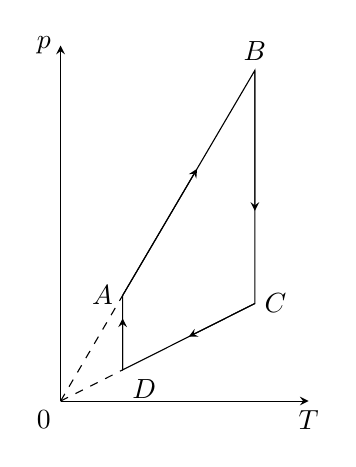
\begin{tikzpicture}[>=stealth,scale=1.05]
\draw[->] (0,0)--(3,0) node[below] {$T$};
\draw[->] (0,0)--(0,4.3) node[left] {$p$};
\node[below left] at (0,0) {$0$};
\coordinate (A) at (.75,{4*.75/2.35});
\coordinate (B) at (2.35,4.0);
\coordinate (C) at (2.35,1.18);
\coordinate (D) at (.75,{1.18*.75/2.35});
\draw[dashed] (0,0)--(A);
\draw[dashed] (0,0)--(D);
\draw (A)--(B)--(C)--(D)--cycle;
\draw[->] (A)--(1.65,{4*1.65/2.35});
\draw[->] (B)--(2.35,2.3);
\draw[->] (C)--(1.55,{1.18*1.55/2.35});
\draw[->] (D)--(.75,1.0);
\node[left] at (A) {$A$};
\node[above] at (B) {$B$};
\node[right] at (C) {$C$};
\node[below right] at (D) {$D$};
\end{tikzpicture}
\end{center}
На рисунке показан график циклического процесса, проведённого с одноатомным идеальным газом, в координатах $p$--$T$, где $p$ --- давление газа, $T$ --- абсолютная температура газа. Количество вещества газа постоянно.
\begin{enumerate}
\item Газ за цикл совершает положительную работу.
\item В процессе $AB$ газ получает положительное количество теплоты.
\item В процессе $BC$ внутренняя энергия газа уменьшается.
\item В процессе $CD$ над газом совершают работу внешние силы.
\item В процессе $DA$ газ изотермически расширяется.
\end{enumerate}
}{
\smallskip\noindent\textbf{Решение от GPT}\par
Из $pV=\nu RT$ следует, что $AB$ и $CD$ --- изохоры, причём $V_{AB}<V_{CD}$. Участки $BC$ и $DA$ --- изотермы, $T_{BC}>T_{DA}$.
\begin{enumerate}
\item Верно: работа за цикл $A_{\text{ц}}=\nu R(T_{BC}-T_{DA})\ln(V_{CD}/V_{AB})>0$.
\item Верно: на $AB$ температура растёт, работа равна нулю, поэтому $Q=\Delta U=\frac32\nu R\Delta T>0$.
\item Неверно: на $BC$ температура постоянна, поэтому $\Delta U=0$.
\item Неверно: на изохоре $CD$ работа равна нулю.
\item Неверно: на $DA$ давление растёт при постоянной температуре, следовательно, газ сжимается.
\end{enumerate}
\textbf{Ответ: 12.}
}

% Source 559e5c: https://ege.fipi.ru/bank/questions.php?search=1&proj=BA1F39653304A5B041B656915DC36B38&qid=559e5c
\BankTask{559e5c}{
\begin{center}
\begin{tikzpicture}[>=stealth,scale=1.1]
\draw[->] (0,0)--(4,0) node[below] {$\overline{E}_{\text{к}}$};
\draw[->] (0,0)--(0,3.35) node[left] {$p$};
\node[below left] at (0,0) {$0$};
\coordinate (one) at (1.25,.7);
\coordinate (two) at (2.65,1.48);
\coordinate (three) at (2.65,3.0);
\draw[dashed] (0,0)--(one);
\draw (one)--(two)--(three);
\draw[->] (one)--(2.1,1.17);
\draw[->] (two)--(2.65,2.5);
\fill (one) circle (1.5pt) node[below right] {$1$};
\fill (two) circle (1.5pt) node[right] {$2$};
\fill (three) circle (1.5pt) node[right] {$3$};
\end{tikzpicture}
\end{center}
Один моль аргона участвует в процессе $1$--$2$--$3$, представленном на графике зависимости давления $p$ от средней кинетической энергии $\overline{E}_{\text{к}}$ теплового движения молекул.
\begin{enumerate}
\item В процессе $1$--$2$ концентрация аргона остаётся неизменной.
\item В процессе $1$--$2$ аргон отдаёт положительное количество теплоты.
\item В процессе $2$--$3$ аргон изотермически расширяется.
\item В процессе $2$--$3$ аргон отдаёт окружающей среде положительное количество теплоты.
\item В процессе $2$--$3$ температура аргона растёт.
\end{enumerate}
}{
\smallskip\noindent\textbf{Решение от GPT}\par
Используем $p=\frac23 n\overline{E}_{\text{к}}$ и $\overline{E}_{\text{к}}=\frac32 kT$.
\begin{enumerate}
\item Верно: на $1$--$2$ отношение $p/\overline{E}_{\text{к}}$ постоянно, следовательно, концентрация $n$ постоянна.
\item Неверно: $1$--$2$ --- изохорное нагревание, $Q=\Delta U>0$, газ получает теплоту.
\item Неверно: на $2$--$3$ температура постоянна, давление растёт, поэтому объём уменьшается: происходит сжатие.
\item Верно: при изотермическом сжатии $\Delta U=0$, работа газа $A<0$, поэтому $Q=A<0$.
\item Неверно: на $2$--$3$ средняя кинетическая энергия и температура постоянны.
\end{enumerate}
\textbf{Ответ: 14.}
}

% Source 196De7: https://ege.fipi.ru/bank/questions.php?search=1&proj=BA1F39653304A5B041B656915DC36B38&qid=196De7
\BankTask{196De7}{
\begin{center}
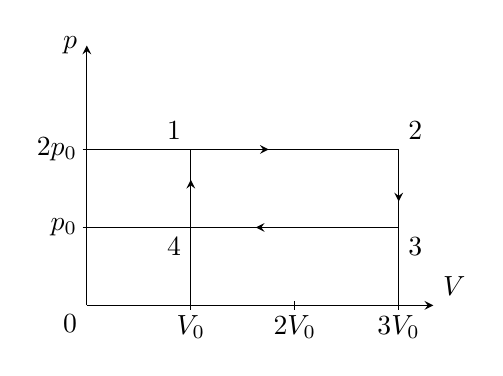
\begin{tikzpicture}[>=stealth,scale=1.1]
\draw[->] (0,0)--(4.0,0) node[above right] {$V$};
\draw[->] (0,0)--(0,3.0) node[left] {$p$};
\node[below left] at (0,0) {$0$};
\draw (0,.9)--(1.2,.9);
\draw (0,1.8)--(1.2,1.8);
\draw (1.2,0)--(1.2,.9);
\draw (3.6,0)--(3.6,.9);
\draw (1.2,.9)--(1.2,1.8)--(3.6,1.8)--(3.6,.9)--cycle;
\draw[->] (1.2,.9)--(1.2,1.45);
\draw[->] (1.2,1.8)--(2.1,1.8);
\draw[->] (3.6,1.8)--(3.6,1.2);
\draw[->] (3.6,.9)--(1.95,.9);
\foreach \x in {1.2,2.4,3.6}\draw (\x,-.05)--(\x,.05);
\foreach \y in {.9,1.8}\draw (-.05,\y)--(.05,\y);
\node[left] at (0,.9) {$p_0$};
\node[left] at (0,1.8) {$2p_0$};
\node[below] at (1.2,0) {$V_0$};
\node[below] at (2.4,0) {$2V_0$};
\node[below] at (3.6,0) {$3V_0$};
\node[above left] at (1.2,1.8) {$1$};
\node[above right] at (3.6,1.8) {$2$};
\node[below right] at (3.6,.9) {$3$};
\node[below left] at (1.2,.9) {$4$};
\end{tikzpicture}
\end{center}
Один моль аргона является рабочим телом в тепловом двигателе, который работает по циклу, показанному на рисунке в переменных $p$--$V$ ($p$ --- давление аргона, $V$ --- его объём).
\begin{enumerate}
\item Аргон получает положительное количество теплоты от нагревателя только в процессе $1$--$2$.
\item В процессе $3$--$4$ внутренняя энергия аргона не изменяется.
\item Работа аргона за цикл равна $2p_0V_0$.
\item В процессе $4$--$1$ аргон отдаёт холодильнику положительное количество теплоты.
\item Максимальная абсолютная температура аргона в цикле в $6$ раз больше минимальной.
\end{enumerate}
}{
\smallskip\noindent\textbf{Решение от GPT}\par
Для одного моля аргона $T=pV/R$, $U=\frac32RT$, $Q=\Delta U+A$.
\begin{enumerate}
\item Неверно: теплота поступает на $1$--$2$ и на $4$--$1$; в обоих процессах температура растёт.
\item Неверно: на $3$--$4$ произведение $pV$ уменьшается, поэтому $\Delta U<0$.
\item Верно: работа за цикл равна площади прямоугольника, $A_{\text{ц}}=(2p_0-p_0)(3V_0-V_0)=2p_0V_0$.
\item Неверно: на $4$--$1$ объём постоянен, температура растёт, поэтому $Q=\Delta U>0$.
\item Верно: максимальная температура достигается в точке $2$, минимальная --- в точке $4$; $T_2/T_4=(2p_0\cdot3V_0)/(p_0V_0)=6$.
\end{enumerate}
\textbf{Ответ: 35.}
}

% Source 1F4F09: https://ege.fipi.ru/bank/questions.php?search=1&proj=BA1F39653304A5B041B656915DC36B38&qid=1F4F09
\BankTask{1F4F09}{
На рисунке показан график циклического процесса, проведённого с одноатомным идеальным газом, в координатах \(V\)–\(T\), где \(V\) — объём газа, \(T\) — абсолютная температура газа. Количество вещества газа постоянно.
\begin{center}
\begin{tikzpicture}[>=stealth,scale=0.95]
\draw[->] (0,0)--(4.7,0) node[below] {$T$};
\draw[->] (0,0)--(0,4.2) node[left] {$V$};
\node[below left] at (0,0) {$0$};
\coordinate (A) at (0.9,1.55);
\coordinate (B) at (1.8,3.1);
\coordinate (C) at (3.25,3.1);
\coordinate (D) at (0.9,0.86);
\draw[dashed,thin] (0,0)--(A) (0,0)--(D);
\draw (A)--(B)--(C)--(D)--(A);
\draw[->] (1.25,2.15)--(1.48,2.55);
\draw[->] (2.25,3.1)--(2.6,3.1);
\draw[->] (2.38,2.27)--(2.02,1.93);
\draw[->] (0.9,1.02)--(0.9,1.35);
\node[left] at (A) {$A$};
\node[above] at (B) {$B$};
\node[above right] at (C) {$C$};
\node[below right] at (D) {$D$};
\end{tikzpicture}
\end{center}
\begin{enumerate}
\item Давление газа в процессе \(CD\) постоянно, при этом над газом совершается положительная работа.
\item В процессе \(DA\) давление газа увеличивается.
\item В процессе \(AB\) газ получает положительное количество теплоты.
\item В состоянии \(D\) концентрация атомов газа максимальна.
\item В процессе \(BC\) внутренняя энергия газа уменьшается.
\end{enumerate}
}{
\smallskip\noindent\textbf{Решение от GPT}\par
Используем \(p=\nu RT/V\), \(U=\frac32\nu RT\), \(n=N/V\).
\begin{enumerate}
\item Верно: участок \(CD\) лежит на прямой, проходящей через начало координат, поэтому \(p=\mathrm{const}\). Объём уменьшается, работа над газом положительна.
\item Неверно: при \(T=\mathrm{const}\) объём на участке \(DA\) растёт, поэтому давление уменьшается.
\item Верно: на участке \(AB\) температура и объём увеличиваются, следовательно, \(\Delta U>0\), \(A>0\) и \(Q=\Delta U+A>0\).
\item Верно: в состоянии \(D\) объём минимален, поэтому концентрация максимальна.
\item Неверно: на участке \(BC\) температура растёт, поэтому внутренняя энергия увеличивается.
\end{enumerate}
\(\boxed{134}\).
}

% Source F72E75: https://ege.fipi.ru/bank/questions.php?search=1&proj=BA1F39653304A5B041B656915DC36B38&qid=F72E75
\BankTask{F72E75}{
На рисунке представлены графики зависимости температуры \(t\) двух тел одинаковой массой от сообщённого им количества теплоты \(Q\). Каждое тело находится в сосуде под поршнем. Первоначально тела находились в жидком агрегатном состоянии.
\begin{center}
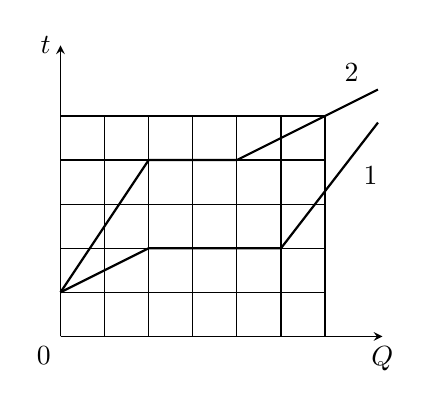
\begin{tikzpicture}[>=stealth,x=0.56cm,y=0.56cm]
\draw[step=1,thin] (0,0) grid (6,5);
\draw[->] (0,0)--(7.3,0) node[below] {$Q$};
\draw[->] (0,0)--(0,6.6) node[left] {$t$};
\node[below left] at (0,0) {$0$};
\draw[thick] (0,1)--(2,2)--(5,2)--(7.2,4.85);
\draw[thick] (0,1)--(2,4)--(4,4)--(7.2,5.6);
\node[right] at (6.65,3.65) {$1$};
\node[above] at (6.6,5.55) {$2$};
\end{tikzpicture}
\end{center}
\begin{enumerate}
\item Температура кипения первого тела в \(2\) раза меньше, чем температура кипения второго тела.
\item Тела имеют одинаковую удельную теплоёмкость в газообразном состоянии.
\item Удельная теплоёмкость в жидком агрегатном состоянии у второго тела в \(3\) раза меньше, чем у первого.
\item Оба тела имеют одинаковую удельную теплоту парообразования.
\item Для первого тела удельная теплоёмкость в жидком агрегатном состоянии меньше удельной теплоёмкости в газообразном состоянии.
\end{enumerate}
}{
\smallskip\noindent\textbf{Решение от GPT}\par
При нагревании \(c=\Delta Q/(m\Delta t)\), при кипении \(L=\Delta Q/m\). Массы одинаковы.
\begin{enumerate}
\item Верно: горизонтальные участки расположены на уровнях \(2\) и \(4\) клеток от нуля температуры, поэтому \(t_{\text{кип},1}=t_{\text{кип},2}/2\).
\item Неверно: наклоны участков нагревания пара различаются, следовательно, теплоёмкости различны.
\item Верно: при одинаковом количестве теплоты на начальных участках \(\Delta t_1=1\) клетка, \(\Delta t_2=3\) клетки. Поэтому \(c_2=c_1/3\).
\item Неверно: длины участков кипения равны \(3\) и \(2\) клеткам по оси \(Q\), поэтому \(L_1/L_2=3/2\).
\item Неверно: участок нагревания пара первого тела круче участка нагревания жидкости, поэтому \(c_{\text{газ},1}<c_{\text{ж},1}\).
\end{enumerate}
\(\boxed{13}\).
}

% Source 4DBED7: https://ege.fipi.ru/bank/questions.php?search=1&proj=BA1F39653304A5B041B656915DC36B38&qid=4DBED7
\BankTask{4DBED7}{
\begin{center}
\begin{tikzpicture}[>=stealth,x=0.85cm,y=0.85cm]
\draw[->] (0,0)--(4.5,0) node[below] {$t$};
\draw[->] (0,0)--(0,2.8) node[left] {$n$};
\node[below left] at (0,0) {$0$};
\draw[thick] (0,0.48) .. controls (0.65,1.2) and (1.15,1.85) .. (1.9,1.85)--(4.05,1.85);
\node at (0.65,1.7) {$1$};
\node at (2.8,2.23) {$2$};
\end{tikzpicture}
\end{center}
В стеклянную колбу налили немного воды и герметично закрыли её пробкой. Вода постепенно испарялась. На рисунке показан график изменения со временем \(t\) концентрации \(n\) молекул водяного пара внутри колбы. Температура в колбе в течение всего времени проведения опыта оставалась постоянной.

В конце опыта в колбе ещё оставалась вода.
\begin{enumerate}
\item На участке \(1\) плотность водяных паров уменьшалась.
\item На участке \(2\) давление водяных паров не менялось.
\item На участке \(1\) водяной пар ненасыщенный, а на участке \(2\) насыщенный.
\item На участке \(1\) давление водяных паров уменьшалось.
\item На участке \(2\) плотность водяных паров увеличивалась.
\end{enumerate}
}{
\smallskip\noindent\textbf{Решение от GPT}\par
При постоянной температуре \(p=nkT\), а плотность пара \(\rho=m_0n\), где \(m_0\) — масса молекулы воды.
\begin{enumerate}
\item Неверно: на участке \(1\) концентрация и плотность растут.
\item Верно: на участке \(2\) концентрация постоянна, поэтому давление не меняется.
\item Верно: на участке \(1\) пар ещё ненасыщенный; на участке \(2\) устанавливается равновесие с оставшейся водой, пар насыщенный.
\item Неверно: на участке \(1\) давление растёт вместе с концентрацией.
\item Неверно: на участке \(2\) плотность постоянна.
\end{enumerate}
\(\boxed{23}\).
}

% Source E2B7DC: https://ege.fipi.ru/bank/questions.php?search=1&proj=BA1F39653304A5B041B656915DC36B38&qid=E2B7DC
\BankTask{E2B7DC}{
В начальный момент в сосуде под лёгким поршнем находится только жидкий эфир. На рисунке схематично представлен график зависимости температуры \(t\) эфира от времени \(\tau\) его нагревания и последующего охлаждения.
\begin{center}
\begin{tikzpicture}[x=0.85cm,y=0.65cm,>=stealth]
\draw[->] (0,0)--(6.8,0) node[below] {$\tau$};
\draw[->] (0,0)--(0,4.7) node[left] {$t,\,{}^\circ\mathrm{C}$};
\node[below left] at (0,0) {$0$};
\foreach \y/\v in {1/20,2/40,3/60}{\draw (-0.08,\y)--(0.08,\y);\node[left] at (-0.1,\y) {$\v$};}
\foreach \y in {0.5,1.5,2.5}{\draw (-0.06,\y)--(0.06,\y);}
\draw[dashed] (0,2)--(3.35,2);
\draw (0,1)--(0.75,2)--(2.1,2)--(2.72,3.4)--(3.35,2)--(4.7,2)--(5.35,1);
\node[below right] at (0,1) {$A$};
\node[above] at (0.75,2) {$B$};
\node[above left] at (2.1,2) {$C$};
\node[above] at (2.72,3.4) {$D$};
\node[above right] at (3.35,2) {$E$};
\node[above right] at (4.7,2) {$F$};
\node[right] at (5.35,1) {$G$};
\end{tikzpicture}
\end{center}
\begin{enumerate}
\item Температура кипения эфира равна \(60\,{}^\circ\mathrm{C}\).
\item В точке \(F\) в сосуде находился только жидкий эфир.
\item На участке \(BC\) внутренняя энергия эфира увеличивалась.
\item В точке \(G\) эфир отвердел.
\item Время, за которое весь эфир выкипел, меньше, чем время, за которое он сконденсировался.
\end{enumerate}
}{
\smallskip\noindent\textbf{Решение от GPT}\par
1) Неверно: горизонтальный участок $BC$ соответствует кипению при $40\,{}^\circ\text{C}$.

2) Верно: в точке $F$ конденсация завершилась, далее охлаждается жидкость.

3) Верно: при кипении внутренняя энергия увеличивается за счёт увеличения потенциальной энергии взаимодействия молекул.

4) Неверно: участок $FG$ соответствует охлаждению жидкости; признаков отвердевания нет.

5) Неверно: участки $BC$ и $EF$ на схематическом графике имеют одинаковую длительность.

Ответ: $23$.
}

% Source 0D668C: https://ege.fipi.ru/bank/questions.php?search=1&proj=BA1F39653304A5B041B656915DC36B38&qid=0D668C
\BankTask{0D668C}{
\begin{center}
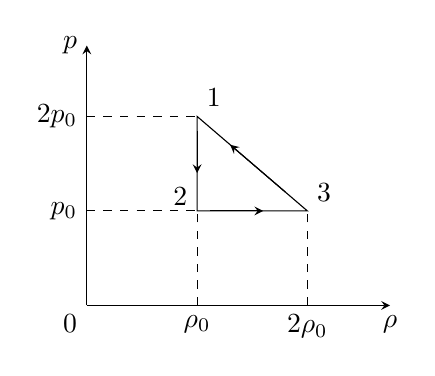
\begin{tikzpicture}[x=1.4cm,y=1.2cm,>=stealth]
\draw[->] (0,0)--(2.75,0) node[below] {$\rho$};
\draw[->] (0,0)--(0,2.75) node[left] {$p$};
\node[below left] at (0,0) {$0$};
\draw[dashed] (0,2)--(1,2);
\draw[dashed] (0,1)--(1,1);
\draw[dashed] (1,0)--(1,1);
\draw[dashed] (2,0)--(2,1);
\node[left] at (0,1) {$p_0$};
\node[left] at (0,2) {$2p_0$};
\node[below] at (1,0) {$\rho_0$};
\node[below] at (2,0) {$2\rho_0$};
\draw (1,2)--(1,1)--(2,1)--cycle;
\draw[->] (1,1.85)--(1,1.4);
\draw[->] (1.12,1)--(1.6,1);
\draw[->] (1.8,1.2)--(1.3,1.7);
\node[above right] at (1,2) {$1$};
\node[left] at (1,1.15) {$2$};
\node[above right] at (2,1) {$3$};
\end{tikzpicture}
\end{center}
\(1\,\text{моль}\) одноатомного идеального газа совершает цикл \(1-2-3-1\), при котором давление \(p\) газа изменяется с изменением плотности \(\rho\) газа так, как показано на рисунке. Значения плотности и давления в вершинах цикла представлены на графике.
\begin{enumerate}
\item Работа газа в процессе \(1-2\) равна нулю.
\item В процессе \(3-1\) газ отдаёт положительное количество теплоты.
\item Температура газа в состоянии \(3\) минимальна.
\item Внутренняя энергия газа в процессе \(2-3\) увеличивается.
\item При переходе газа из \(3\) в \(1\) внутренняя энергия не меняется.
\end{enumerate}
}{
\smallskip\noindent\textbf{Решение от GPT}\par
Для неизменной массы газа \(V=m/\rho\), \(T=Mp/(R\rho)\), где \(M\) — молярная масса. Обозначим \(T_0=Mp_0/(R\rho_0)\). Тогда
\[
T_1=2T_0,\qquad T_2=T_0,\qquad T_3=\frac{T_0}{2},\qquad U=\frac32\nu RT.
\]
1) Верно: \(\rho=\mathrm{const}\), следовательно, \(V=\mathrm{const}\) и \(A_{12}=0\).

2) Неверно: при переходе \(3\to1\) газ расширяется, \(A_{31}>0\), и нагревается, \(\Delta U_{31}>0\). Поэтому \(Q_{31}=\Delta U_{31}+A_{31}>0\): газ получает теплоту.

3) Верно: \(T_3<T_2<T_1\).

4) Неверно: \(T_3<T_2\), поэтому \(\Delta U_{23}<0\).

5) Неверно: \(T_1>T_3\), поэтому \(\Delta U_{31}>0\).

Ответ: \(13\).
}

\end{document}
